\chapter{Experiments}
\label{c:experiments} To evaluate different versions of collaborative filtering algorithms and compare their performance to social collaborative filtering algorithms, simulations were run with the help of software designed specifically for this purpose. This chapter explains the experiments that were conducted and explains and interprets the results. The five basic experiments were:

\begin{enumerate}
\item Different versions of user-based collaborative filtering are evaluated on the last.fm dataset.
\item Different versions of social user-based collaborative filtering are evaluated on the last.fm dataset and compared to the conventional ones.
\item Different artificially generated networks and ratings are used to again compare collaborative filtering and social collaborative filtering and find conditions under which social collaborative filtering might perform better.
\item The hypothesis that central users in communities might be better predictors was analyzed.
\item The hypothesis that social collaborative filtering works better for certain users was analyzed.
\end{enumerate}

\section{Experimental Setup}
\label{st:experimentalsetup}

\subsection{Last.fm Dataset}
\label{sst:lastfmdataset} The dataset from last.fm is publicly available and can be obtained from the ``Social Computing Research at the University of Minnesota'' website \cite{Grouplens}. It contains information about 1892 (anonymized) users and 17632 artists. Since the users on last.fm do not explicitly give ratings to an artist, the degree to which a user likes or dislikes an artist is expressed as ``listening-count'' (how many times a user has listened to an artist). There are 92'834 $(user, artist, listeningcount)$-tuples. The dataset further contains 12'717 bi-directional user friend relations in the form of $(user_i, user_j)$-pairs. The dataset further also contains informations about tags that users assigned to artists, but these will not be used in the experiments. However, the friend relations will be used and are indeed very important for the social collaborative filtering algorithms.

\subsubsection{Normalization and cleaning-up of the Dataset}
\label{sst:normalizationandcleaningup} The rating file consisting of $(user, artist, listeningcount)$-tuples can already be used as input for a recommender algorithm. With k-fold cross-validation, the tuples can be partitioned into training and test sets. The problem is that the performance of the algorithms will be quite hard to evaulate, since the RMSE that is often used to measure the performance largely depends on the range of the ratings. The listeningcounts that are used as ratings in the last.fm dataset range from 1 to 352'698. There are users who have listeningcounts in the range of a couple of dozen, and others that only have listeningcounts beyond 1'000. This suggests that the listeningcounts need to be normalized so that the resulting RMSE's can acually be interpreted to make statements about the performance of the recommender algorithms.

There are a few steps in the normalization and clean-up process. Firstly, the few users that have the same listeningcount 1 for every artist they have listened to are completely removed. There is no information about the preferences of those users contained in their ratings. It is justifiable to do this since real recommender systems will hardly ever have to deal with a user that gives every item the same rating. Secondly, users with less than 10 ratings are also removed. This is done because of the partitioning of the dataset into training and test sets. There should always be users in both the partitioning and the training set, even if k is as high as 10.

After these removals have been performed, the listeningcounts need to be normalized in the following way:
\newline

\begin{algorithm}[H]
\SetAlgoLined
\KwData{All $(user,artist,listeningcount)$-tuples $x=(u,a,l) \in X$, min (e.g. 1), max (e.g. 5)}
\KwResult{Normalized $(user,artist,rating)$-tuples $x'=(u,a,r) \in X'$ with $r$ between min and max}
\For{$u \in X$}{
currentMin = findMinimum(u)\;
currentMax = findMaximum(u)\;
\For{each $x$ with $x(u)=u$}{
normalizingFactor = $\frac{x(l) - currentMin}{currentMax - currentMin}$\;
r = $normalizingFactor \cdot (max-min) + min$\;
$x'=(u,a,r)$\;
}
}
\caption{Normalize Ratings}
\end{algorithm}

After this algorithm is run, all ratings are in the range $[min,max]$ and are suited as input for the recommender algorithms. As a consequence, the friend relations also need to be updated. All relations containing one of the users removed beforehand are also removed. This leaves us with 92'770 of the original 92'834 ratings and 12'508 of the original 12'717 friend relations.

\subsection{k-fold cross-validation}
\label{kfoldcrossvalidation} Cross-validation is a technique used in statistical analysis to evaluate the accuracy of a prediction model on a given dataset. The dataset is partitioned into a training set, which will be used to ``train'' the model or algorithm, and a test set, which will be used to measure the prediction accuracy.

In k-fold cross-validation, the dataset is randomly split into $k$ subsets of equal size. One of the subsets will serve as the test set and the other $k-1$ will be used as the training set. This is repeated $k$ times, with each subset serving as test set exactly once. This method has the advantage over completely random splitting that each data point is guaranteed to be used in the test set (exacty once).

\section{Experiment 1}
\label{st:experiment1} The first experiment was run on the normalized last.fm dataset with the goal of comparing the performance of different versions of user-based collaborative filtering algorithms. In this particular setting, item-based collaborative filtering was not practicable. Calculating all user-user similarities for around 1'800 users (around 3'250'000 similarities) takes almost 100 times less time than calculating all item-item similarities for around 17'500 items (around 306'250'000 similarities), actually resulting in equal or even better performance.

The dataset was split using 5-fold cross-validation. To adjust the cross-validation to this particular setting, the process was adjusted a little. Instead of randomly partitioning the 92'770 ratings into 5 subsets, this was done for every user's ratings seperately. This extra step was taken to ensure that for every user there is training data as well as test data.

The two different similarity measures and the three prediction measures presented in \ref{ssst:userbasedcf} were tested in all possible combinations. The neighbourhood sizes were determined either by a fixed number $n$ (from 1 up to all users) or a similarity threshold $\lambda$ was applied (from 0.0 to 1.0). All resulting parameter combinations were applied to the 5-fold cross-validated dataset, and this was done 5 times, resulting in 25 runs for each parameter setting. The resulting RMSE's were averaged over those 25 runs. The results can be seen in \ref{f:userbasedn} and \ref{f:userbasedt}.

\begin{figure}[!ht]
\centering
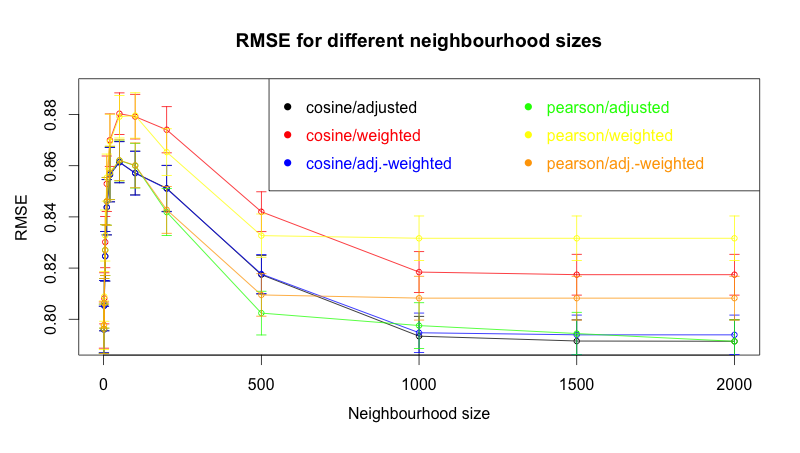
\includegraphics[width=400px]{./4-experiments/figures/USERBASED_N_V3.png}
\label{f:userbasedn}
\caption{Results for neighbourhood}
\end{figure}

\begin{figure}[!ht]
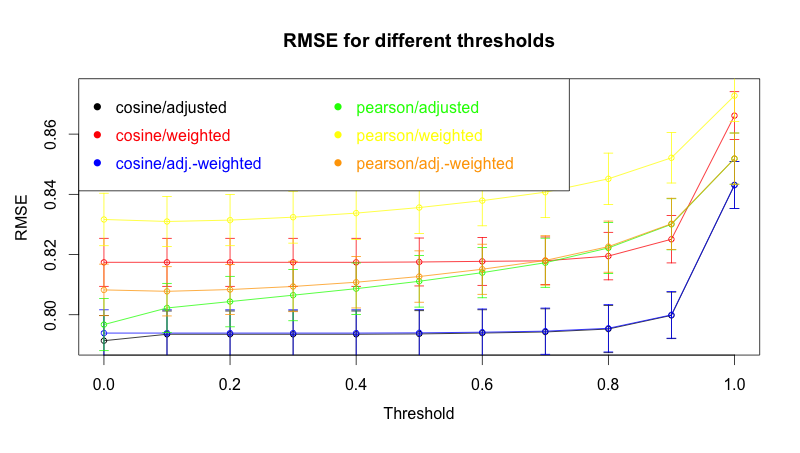
\includegraphics[width=400px]{./4-experiments/figures/USERBASED_T_V3.png}
\label{f:userbasedt}
\caption{Results for threshold}
\end{figure}

It can be seen that the differences between the different similarity measure/prediction measure combinations are relatively small. Overall, the combinations of using the cosine similarity and the adjusted-weighted sum performs best. Looking at the prediction measures, one can quickly conclude that the consideration of the average rating of a user (as done by the adjusted sum) is more important and makes the predictions more accurate than the consideration of the weights. In fact, the adjusted sum performs almost as good as the adjusted-weighted sum.

Two things stand out: The peak at neighbourhood $n=50$ and the peak at threshold $\lambda = 1.0$. At first sight, this is quite astonishing, since other studies have shown a local optimum at neighbourhoods of around 50. It seems weird that there is no such minimum, but instead a clear maximum. To explain these effects, one important realization is to understand that the size $n$ of the neighbourhood $N$ is not necessarily equal to the number of users included in the prediction calculation. As explained in \ref{ssst:userbasedcf}, out of all users in $N$, only the ones who have actually rated item $j$ can be included in the calculation. In sparse rating matrices, chances are that the actual set of users included in the prediction calculation is much smaller than $n$. As for the last.fm dataset, with 1'873 users and 17'612 items after normalization, there are 32'987'276 possible ratings of which only 92'770 are actually provided. The rating matrix thus has a density of only 0.3 \% or a sparsity of 99.7 \%. The results suggest that in a setting with very sparse rating matrices, larger neighbourhoods should be chosen so that enough users are included in the prediction.

The dataset of last.fm has another characteristic that amplifies this effect: There are many items that have only received one rating. Of course, when the rating for one of these items falls into the test set and has to be predicted, there is no possible information from other users' ratings to take into account. In this case, the algorithm chooses as prediction just the average rating of user $i$ over all his ratings. The experiments showed that the average had to serve as prediction in over half of the predictions for a fixed neighbourhood of size 70 (with an average of only 1.87 users per prediction that had actually rated the item). The average of users actually included in the prediction hit 50 at $n = 1050$. When a threshold on the similarities is applied, the actual neighbourhoods are much larger, which explains the constantly low RMSE's. Only with a threshold of 1.0, the average of users actually included sinks drastically to 9, which explains the decrease in performance.